Podle literatury \cite{19} se v telekomunikacích používají filtry v rozsahu kmitočtů desítek až stovek MHz, v bezdrátové komunikaci až v řádu GHz. Běžné RC filtry by neměly být užívány ve frekvenčním rozsahu nad 5--10$\%$ $\omega _m$ ($\omega _m = f_m \cdot 2 \pi$, kde $f_m$ je mezní kmitočet) - tedy v tomto rozsahu používaném v telekomunikačních technologiích nemají předvídatelné průběhy. Krom toho ve spínačích CMOS, kde rezistory běžně nejsou dostupné, jsou potřeba zesilovače s velkou šířkou pásma a zároveň vysokým zesílením. Dodržení těchto požadavků je náročné a drahé. Dalším extrémem pro analogové integrované filtry jsou telefonní linky, kde jsou kmitočtové rozsahy sice nízké, ale je požadována nízká cena a vysoká přesnost.\\
\\
Pro nízké frekvence se ke splnění těchto požadavků používají obvody se spínanými kapacitory (SC). Přepínaný kapacitor se chová jako rezistor, tudíž časová konstanta RC je definována poměrem kapacitorů a hodinovou (CLK) frekvencí, se kterou jsou přepínány. Pro vysokofrekvenční aplikace (v řádu GHz) se používají MOSFET-C filtry.\\
\\
Další z možných prvků, které jsou dostupné jak pro nízkofrekvenční aplikace, tak pro kmitočtový rozsah stovek megahertz, jsou transkonduktanční zesilovače. Jejich kmitočtové vlastnosti umožňují využití při konstrukci ARC (\textit{Active RC}) filtrů v pracovním kmitočtovém pásmu do cca 10 MHz a se speciálně konstruovanými OTA až do 100 MHz. Kmitočet dominantního pólu je běžně v oblasti stovek kHz až jednotek MHz (literatura \cite{10}).\\
\\
Transkonduktanční zesilovače (označují se též jako OTA (\textit{Operational Transconductance Amplifiers}) jsou napětím řízené zesilovače s proudovým výstupem - zdroje proudu
\begin{equation}
i_{out} = g_m(u_+ - u_-),
\end{equation}
kde $u_+$ a $u_-$ jsou napětí invertujícího a neinvertujícího vstupu. Transkonduktance je řízena klidovým stejnosměrným pracovním proudem $I_{ABC}$. Ideální OTA má kmitočtově nezávislou transkonduktanci $g_m$ (na rozdíl od reálného, který je kmitočtově závislý). Ideální OTA má také nekonečnou vstupní a výstupní impedanci. S ohledem na proudový (t.j. vysokoimpedanční) výstup OTA je výraznější vliv výstupní impedance. Ta má jak odporovou, tak kapacitní složku a musí být při návrhu ARC obvodů (sekce \ref{s:ARC}) respektována. Vstupní impedance, s ohledem na to, že OTA bývá implementován v CMOS technologii, má převážně kapacitní charakter (literatura \cite{10}).
\begin{figure}[h]
\centering
\includegraphics[scale=0.7]{image7.png}
\caption[OTA - schematické značky]{OTA - schematické značky \cite{11}}
\end{figure}
\begin{figure}[h]
\centering
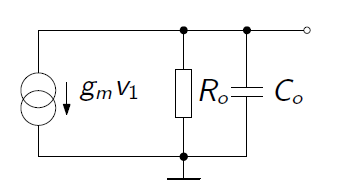
\includegraphics[scale=0.6]{gmrc.png}
\caption[Linearizovaný model reálného OTA]{Linearizovaný model reálného OTA \cite{12}}
\end{figure}
\noindent Připojením zátěže $R_z$ na výstup bylo získáno napětí naprázdno
\begin{equation}\label{s:vzt}
u_{out} = R_zg_m(u_+ - u_-) = G_0(u_+ - u_-),
\end{equation}
kde $G_0$ je zesílení. Ze vztahu \ref{s:vzt} plyne, že zesílení je konečné a mezi vstupy je nenulové napětí. \\
\noindent Po připojení kondenzátoru jako zátěže byl získán bezeztrátový integrátor s přenosem
\begin{equation}
H(s) = \frac{v_2}{v_1} = \frac{g_m}{pC}
\end{equation}
\noindent a napětím na výstupu
\begin{equation}
v_0(t) = \frac{1}{C}\int i(t)dt = \frac{1}{C}\int g_mv_1(t)dt.
\end{equation}
\begin{figure}[h]
\centering
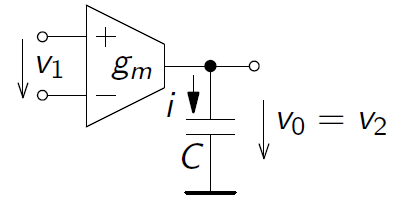
\includegraphics[scale=0.5]{otaintegrator.png}
\caption[OTA-C]{OTA-C \cite{12} \label{s:GM-C}}
\end{figure}
\noindent Toto zapojení integrátoru s uzemněným kondenzátorem se označuje jako OTA-C.\\
\\
Ztrátový integrátor lze utvořit sériovým zapojením dalšího OTA jako odporu se zápornou zpětnou vazbou. Rozdíl mezi ideálním a ztrátovým integrátorem lze pozorovat v modulové charakteristice - pro ztrátový je konstantní a pak teprve lineárně klesá se sklonem -20~dB/dek.\\
Po doplnění ztrátové vodivosti, kterou zde simuluje druhý zesilovač, paralelně k integrační kapacitě, byl obdržen vztah pro výstupní napětí
\begin{equation}
v_0(t) = \frac{g_{m1}}{sC + g_{m2}}(v_1^+ - v_{1}^-).\label{s:OTA-INT1}
\end{equation}
\begin{figure}[h]
\centering
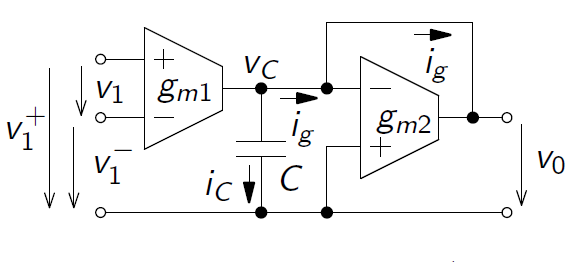
\includegraphics[scale=0.5]{damp.png}
\caption[Ztrátový OTA-C]{Ztrátový OTA-C \cite{12} \label{s:OTA-INT}}
\end{figure}
\subsection{Proudový konvejor druhé generace s OTA}
Podle literatury \cite{15} je jeden z nejzákladnějších bloků v oblasti analogových obvodů v proudovém módu proudový konvejor (\textit{current conveyor (CC)}). Princip CC první generace byl popsán v roce 1968 (K. C. Smith, A. S. Sedra \cite{13}). \textit{CCI} byl následně nahrazen univerzálnější druhou generací v roce 1970 (\textit{CCII})\cite{14}. Obvody s CC se používaly především v zapojeních s bipolárními tranzistory kvůli jejich vysoké transkonduktanci (v porovnání s CMOS). Jsou to operační zesilovače s proudovou zpětnou vazbou (např. MAX477, MAX4112). Proudové konvejory (\textit{Current conveyors}) jsou používány ve vysokofrekvenčních obvodech, kde je problematické použití běžných operačních zesilovačů, protože jsou limitovány násobkem šířky pásma a zesílení (\textit{gain-bandwidth product}). Je to struktura s třemi vstupy.
\begin{figure}[h]
\centering
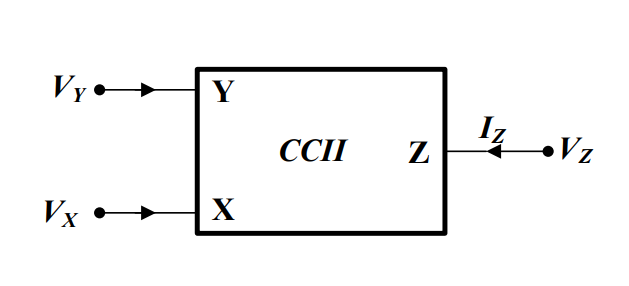
\includegraphics[scale=0.35]{ccii.png}
\caption[CCII symbol]{CCII symbol \cite{15}}
\end{figure}
\noindent Proudovým konvejorem lze také jednoduše realizovat integrátor. Pro výstupní napětí $u_0$ obvodu a z něj odvozenou přenosovou funkci platí
\begin{align}
u_0(t) &= \frac{1}{C}\int i_c(t)dt = \frac{1}{RC}\int u_{in}(t)dt \\
H(p) &= \frac{U_2}{U_1} = \frac{1}{pCR}.
\end{align}
\noindent Konvejorový integrátor pracuje jako invertující nebo neinvertující.
\begin{figure}[h]
\centering
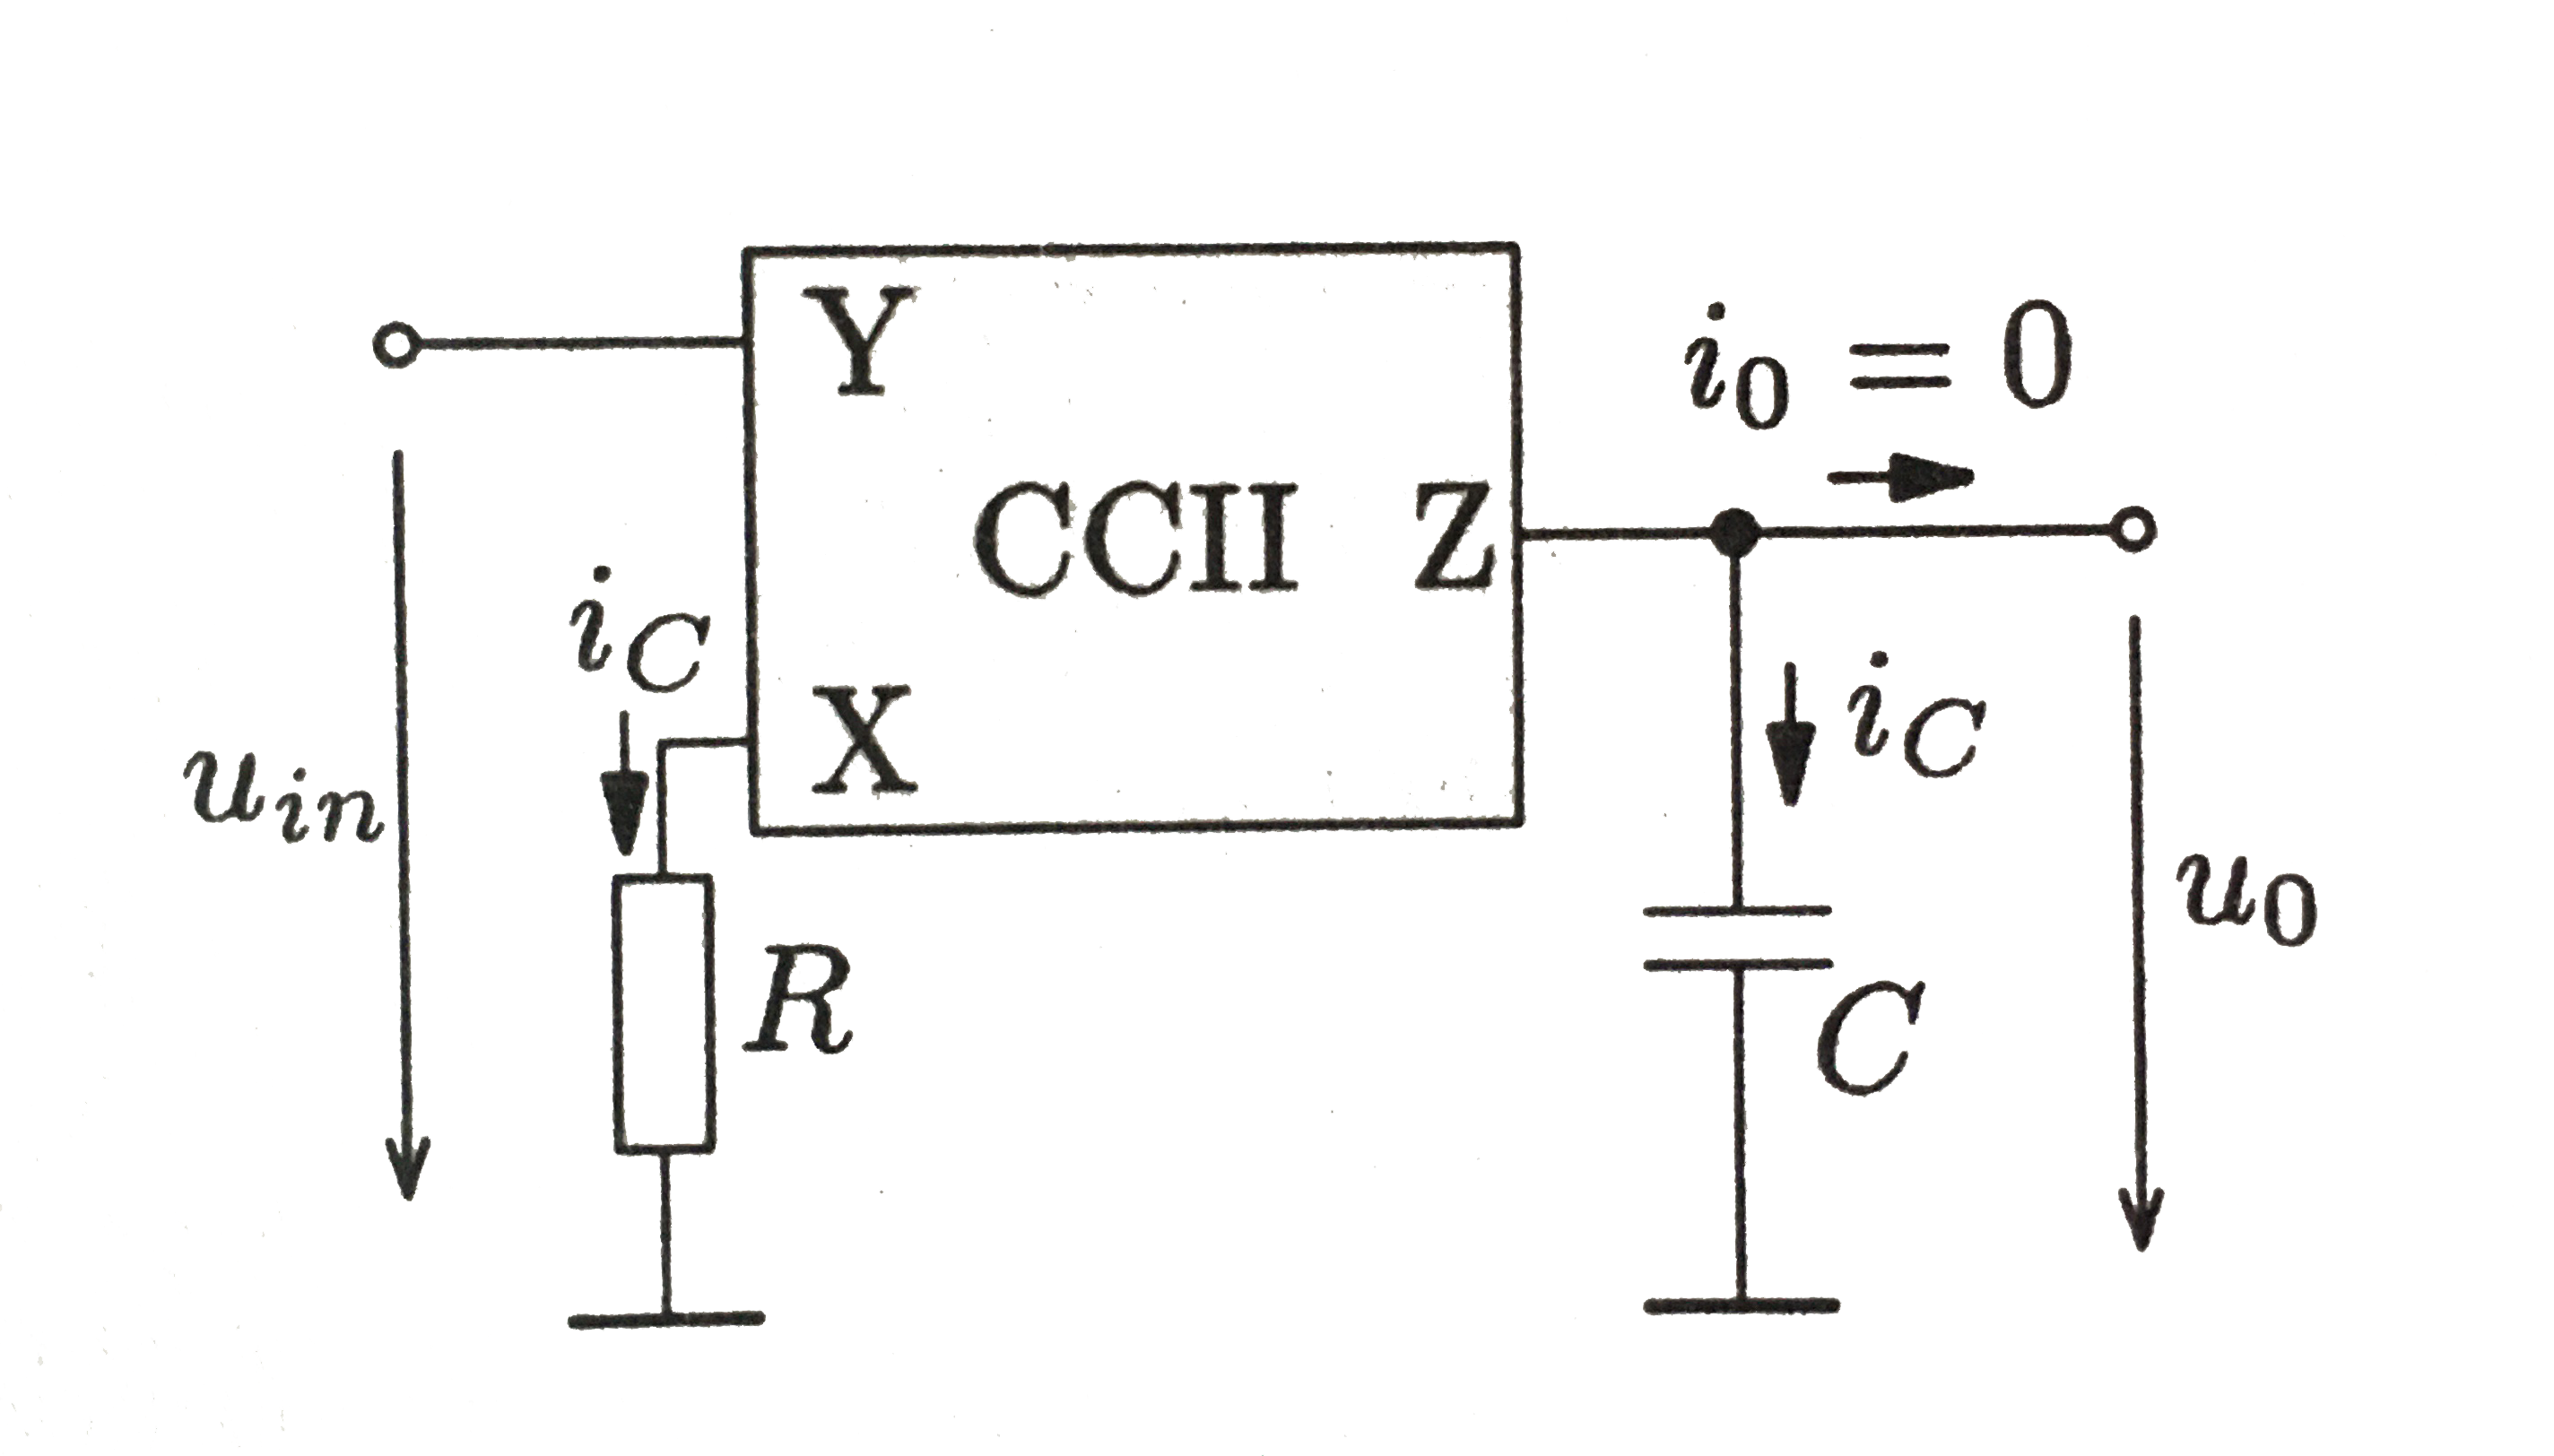
\includegraphics[scale=0.065]{ccii_int1.png}
\caption[Integrátor s CCII a OTA]{Integrátor s CCII a OTA \cite{10}}
\end{figure}
\noindent Vstupní impedance na vstupu Y je nekonečná (tedy proud tekoucí skrz Y je nulový) a impedance na vstupu X je nulová ($R_Y = \infty, I_Y = 0, R_X = 0$). Napětí na vstupu X je ekvivalentní k napětí na vstupu Y ($V_X = V_Y$). Proud procházející vstupem X je ekvivalentní k proudu vstupem Z ($I_Z = I_X$). Výstupní impedance vstupu Z je nekonečná ($R_Z = \infty$).
Charakteristika ideálního \textit{CC} je reprezentována maticí
\begin{equation}
\begin{bmatrix}
I_Y \\ V_X \\ I_Z
\end{bmatrix}
=
\begin{bmatrix}
0 & 0 & 0 \\
1 & 0 & 0 \\
0 & \pm 1 & 0 
\end{bmatrix}
\begin{bmatrix}
V_Y \\
I_X \\
V_Z
\end{bmatrix}.
\end{equation}
\begin{figure}[h]
\centering
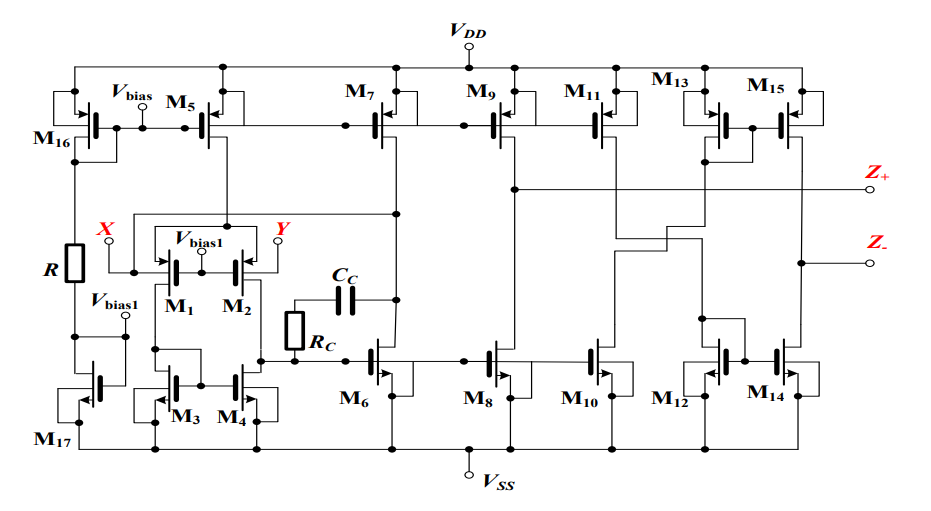
\includegraphics[scale=0.45]{cciiota.png}
\caption[CCII s $\pm$ výstupem založený na OTA]{CCII s $\pm$ výstupem založený na OTA \cite{15}}
\end{figure}
\newline
V analogových IC je preferováno diferenční zpracování signálů, protože redukuje zkreslení a šum (diferenční stupeň vyruší kladné a záporné výchylky napětí/proudu např. na zdroji a také vyruší nelinearity způsobené zesilovačem).\\
Využitím zapojení na obrázku \ref{s:OTA} a principů \textit{CCII} lze získat modifikace klasického transkonduktančního zesilovače (s rozdílovým stupněm na vstupu a jedním výstupem). Obdržené atypické struktury obsahují jeden vstup a jeden výstup a také dva rozdílové stupně (na vstupu i výstupu). Provodení diferenčního stupně na výstupu je znázorněno na obrázku \ref{s:CMOS}. Takovéto zapojení funguje jako dobrý sledovač napětí, ale zato má menší šířku pásma. Také má menší transkonduktanci, protože každou polovinou diferenčního obvodu teče jen polovina klidového stejnosměrného pracovního proudu. Problémem je také relativně nízké stejnosměrné zesílení, proto se v praxi se zapojením s OTA nepoužívá. \\
\begin{figure}[h]
\centering
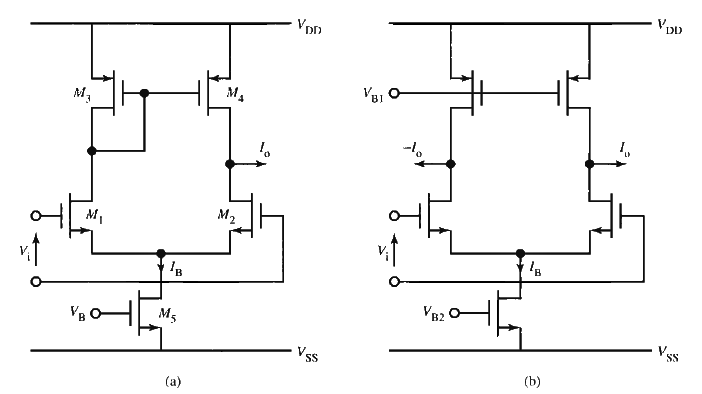
\includegraphics[scale=0.5]{diff.png}
\caption[Základní CMOS transkonduktance a) jeden výstup b) diferenční výstup]{Základní CMOS transkonduktance a) jeden výstup b) diferenční výstup \cite{19} \label{s:CMOS}}
\end{figure}
\begin{figure}[h]
\centering
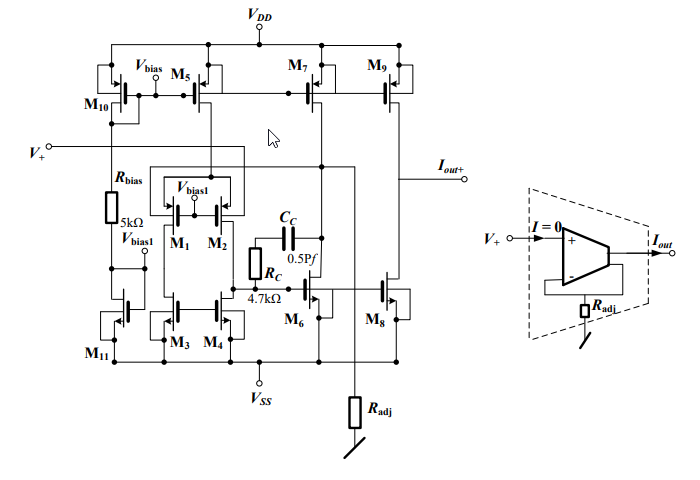
\includegraphics[scale=0.6]{siso.png}
\caption[Single input single output OTA (SISO) založený na CCII]{Single input single output OTA (SISO) založený na CCII \cite{15}}
\end{figure}
\begin{figure}[h]
\centering
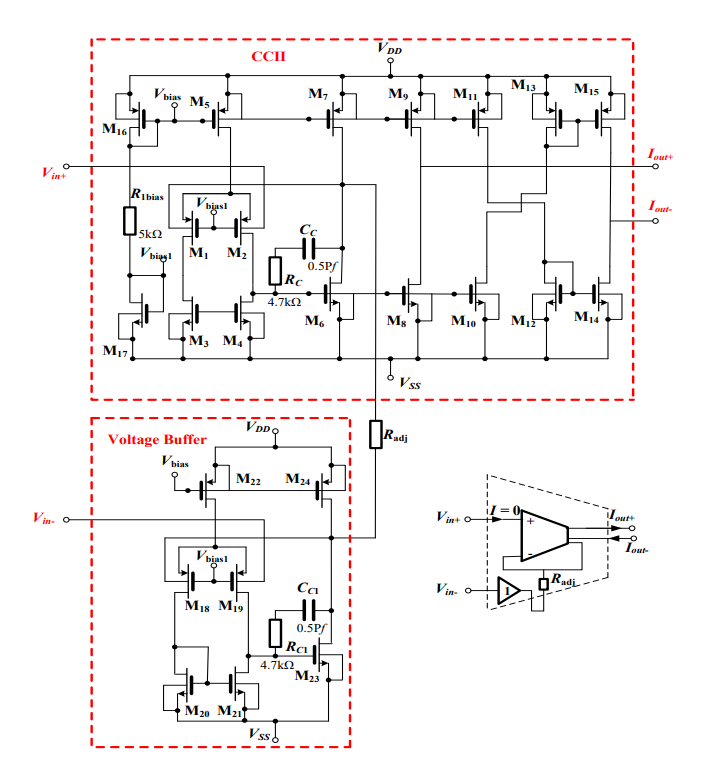
\includegraphics[scale=0.5]{dido.png}
\caption[\textit{Fully differential} OTA (DIDO) založený na CCII a napěťovém bufferu]{\textit{Fully differential} OTA (DIDO) založený na CCII a napěťovém bufferu \cite{15}}
\end{figure}
\newpage
\subsection{IC s OTA}
OTA bývá nejčastěji implementován v unipolární monolitické technologii (CMOS) a v případě, že se jedná o reálný prvek, má převážně kapacitní charakter (vstupní impedance se stává kapacitou). Integrované obvody se vyrábí buď s jedním nebo dvěma zesilovači v pouzdře. Varianty s jedním operačním zesilovačem jsou např. OPA615, OPA860 a novější OPA861. Všechny součástky s jedním OTA mají velkou šířku pásma (v řádech stovek MHz), cenově vychází na 85 -- 290~Kč. IC s dvěma zesilovači v pouzdře mají užší šířku pásma (2 MHz), menší rychlost přeběhu (50 V/$\mu$s), mnohem menší výstupní proud (650 $\mu$A) i offset vstupního napětí a operují při cca 4x nižších proudech. Cenové rozpětí pro pouzdro čipu s 2 OTA je 35 -- 65~Kč. Ceny v tabulce jsou uváděny pro jednu součástku k 10. 11. 2019. Pokud se vyrábí více verzí součástky, je vždy pro přehlednost uvedena pouze jedna. \textit{Gain bandwidth product (GBP)} v tabulce je získán vynásobením hodnoty kmitočtu dominantního pólu celkovým zesílením. Například, podle literatury \cite{11}, je-li navrhován zesilovač se zesílením G, je hodnota mezního kmitočtu pro pokles 3 dB dána vztahem
\begin{equation}
f_m = \frac{GBP}{G}.
\end{equation}
\noindent Pro jednotkové zesílení je hodnota mezního kmitočtu rovna GBP. Někdy se místo GBP udává parametr UGB (\textit{Unity Gain Bandwidth} - šířka pásma při jednotkovém zesílení), který má shodný význam, nebo tranzitní kmitočet $f_T$. Tranzitní kmitočet $f_T$ je kmitočet, na kterém klesne zesílení OZ na 0 dB, tj. na kterém přestává OZ zesilovat. Šířka pásma s útlumem 3 dB je funkcí klidového stejnosměrného pracovního proudu a pro proudy pod 100 $\mu$A je platí přibližně
\begin{equation}
3dB BW = 3 \cdot 10^{11} I_{ABC}.
\end{equation}
\renewcommand{\arraystretch}{1.5}
\begin{table}[h]
\scalebox{0.9}{%
  \begin{tabular}{ | c | >{\centering\arraybackslash}p{1.25cm}| >{\centering\arraybackslash}p{1.25cm} | >{\centering\arraybackslash}p{1.25cm} | >{\centering\arraybackslash}p{1cm} | >{\centering\arraybackslash}p{1cm} | >{\centering\arraybackslash}p{1.25cm} | >{\centering\arraybackslash}p{1.2cm} | >{\centering\arraybackslash}p{1.35cm} |>{\centering\arraybackslash}p{1.2cm} |>{\centering\arraybackslash}p{1cm} |}
    \hline
      & GBP & SR & Výstupní proud na kanál & $I_b$ - vstupní klidový proud & $V_{os}$ - vstupní napěťová nesymetrie & Provozní napájecí proud & Minimální transkonduktance & Napájecí napětí &  Šířka pásma 3 dB & Cena \\ \hline
    OPA615ID & 710 MHz & 2.5 kV/$\mu$s & 5 mA & 3 $\mu$A & 40 mV & 13 mA & 65 mA/V & 8--12.4 V & 710 MHz & 285.22 Kč Kč\\ \hline
    OPA860ID & 470 MHz & 3.5 kV/$\mu$s & 15 mA & 5 $\mu$A & 12 mV & 11.2 mA & 80 mA/V & 5--13 V & 470 MHz & 168.22 Kč\\ \hline
    OPA861ID & 400 MHz & 900 V/$\mu$s & 15 mA & 1 $\mu$A & 12 mV & 5.4 mA & 65 mA/V & 4--12.6 V & 80 MHz & 82.68 Kč\\ \hline
     LT1228CS8\#PBF & 100 MHz & 500 V/$\mu$s & 65 mA & 0.4$\mu$A  & 3 mV & 9 mA  & 0.75 mA/V & 4--36 V & 80 MHz &  210.34 Kč\\
    \hline
  \end{tabular}}
  \caption[Porovnání integrovaných obvodů s jedním OTA]{\label{tab:Porovnání IC s jedním OTA}Porovnání IC s jedním OTA \cite{16}}
  \end{table}
\begin{center}
\begin{table}[h]
\scalebox{0.9}{%
  \begin{tabular}{ | c | >{\centering\arraybackslash}p{1.25cm}| >{\centering\arraybackslash}p{1.25cm} | >{\centering\arraybackslash}p{1.25cm} | >{\centering\arraybackslash}p{1cm} | >{\centering\arraybackslash}p{1cm} | >{\centering\arraybackslash}p{1.3cm} | >{\centering\arraybackslash}p{1.4cm} | >{\centering\arraybackslash}p{1.25cm} |>{\centering\arraybackslash}p{1.25cm} |>{\centering\arraybackslash}p{1cm} |}
    \hline
      & GBP & SR & Výstupní proud na kanál & $I_b$ - vstupní klidový proud & $I_{os}$ - vstupní proudová nesymetrie & Provozní napájecí proud & Minimální transkonduktance & Napájecí napětí & CMMR & Cena \\ \hline
    LM13700M & 2 MHz & 50 V/$\mu$s & 650 $\mu$A & 5 $\mu$A & 4 mV & 1.3 mA & 6700 $\mu$S & 10--36 V & 80--110 dB & 32.50 Kč \\ \hline
    NE5517DG & 2 MHz & 50 V/$\mu$s & 650 $\mu$A & 5 $\mu$A & 5 mV & 2.6 mA & 5400 $\mu$S & 4--44 V & 80 dB & 43.42 Kč \\ \hline
    AU5517DR2G & 2 MHz & 50 V/$\mu$s & 650 $\mu$A & 5 $\mu$A & 5 mV & 2.6 mA & 5400 $\mu$S & 4--44 V & 80 dB & 64.48 Kč \\ \hline
    NJM13600M & 2 MHz & 50 V/$\mu$s & 650 $\mu$A & 5 $\mu$A & 5 mV & 2.6 mA & 6700 $\mu$S & 36 V & 80 dB & 36.92 Kč \\ \hline
    NJM13700M & 2 MHz & 50 V/$\mu$s & 650 $\mu$A & 5 $\mu$A & 4 mV & 2.6 mA & 6700 $\mu$S & 36 V & 80 dB & 37.70 Kč \\ \hline
  \end{tabular}}
  \caption[Porovnání integrovaných obvodů se dvěma OTA]{\label{tab:Porovnání IC se dvěma OTA}Porovnání IC se dvěma OTA \cite{16}}
  \end{table}
\end{center}
\noindent Pro realizaci přeladitelného filtru byl zvolen LM13700M kvůli provoznímu napájecímu proudu (1.3 mA), rozpětí napájecího napětí (10 –- 36 V) a cenové dostupnosti (32.50\ Kč). Součástky NJM13700, NJM13600 a LM13600 se dají zakoupit, ale mají plánované vyřazení z výroby kvůli zastarání. \\
LM13700 má linearizující diody a buffery s diferenciálním vstupem a push-pull výstupem. Dva zesilovače na čipu mají stejné napájení, ale jinak fungují nezávisle na sobě. Linearizační diody snižují zkreslení, a tak umožňují vyšší hodnoty amplitudy vstupního signálu. Výsledkem je zesílení odstupu signál-šum o 10 dB (0.5\% THD). Vysokoimpedanční buffery doplňují dynamický rozsah zesilovače. Výstupní buffery LM13700 se liší od předchozí, již nevyráběné, řady 13600 v tom, že jejich vstupní klidové proudy $I_b$ (a tedy jejich výstupní stejnosměrné úrovně) jsou nezávislé na klidovém stejnosměrném pracovním proudu $I_{ABC}$. To má za následek např. vyšší výkon ve zvukových aplikacích než s LM13600. LM13700 je přeladitelný přes 6 dekád a má výbornou linearitu transkonduktance $g_m$. LM13700 má na výstupu vysokou hodnotu odstupu signál od šumu. Je ekologicky nezávadný a neobsahuje brom (Br) ani antimon (Sb). Nemá vestavěnou ochranu komponentů citlivých na elektrostatický náboj (ESD). Během skladování nebo manipulace by elektrody měly být zkratovány k sobě nebo by se zařízení mělo umístit do vodivé pěny, aby se zabránilo elektrostatickému poškození bran MOS (\cite{18}).\\
Porovnání ceny typů LM13700 je uvedeno v tabulce níže. Parametry jsou stejné, typy se od sebe liší počtem kusů v balení a typem pouzdra (SOIC/PDIP).
\begin{table}[h]
\centering
  \begin{tabular}{ | c | >{\centering\arraybackslash}p{2cm}|>{\centering\arraybackslash}p{2cm}|>{\centering\arraybackslash}p{2cm}|}
    \hline
      & Typ pouzdra & Ks v balení & Cena \\ \hline
    LM13700M/NOPB & SOIC & 48 & 32.50 Kč\\ \hline
    LM13700MX/NOPB & SOIC & 2500 & 27.04 Kč\\ \hline
    LM13700N/NOPB & PDIP & 25 & 48.62 Kč\\ \hline
  \end{tabular}
  \caption[Porovnání typů LM13700]{\label{tab:Porovnání typů LM13700}Porovnání typů LM13700 \cite{16}}
  \end{table}
\begin{figure}[h]
\centering
\includegraphics[scale=0.55]{image6.png}
\caption[Pinout LM13700M]{Pinout LM13700M \cite{17} \label{s:PIN}}
\end{figure}
\noindent Vnitřní zapojení LM13700 na obrázku \ref{s:OTA} obsahuje symetrický rozdílový zesilovací stupeň (tranzistory Q4, Q5), který je napájen řízeným zdrojem proudu s tranzistorem Q2. Tento diferenční stupeň pracuje jako měnič vstupního rozdílového napětí na diferenční proudový signál, který je převeden proudovými zrcadly (\textit{Current Mirror}) na výstupní svorky obvodu. Proudová zrcadla zde tvoří dvojice diod a tranzistorů - referenční proud tekoucí v jedné větvi obvodu se \uv{zrcadlí} ~v jeho druhé větvi. Principiálně jsou to zdroje proudu řízené proudem (viz literatura \cite{20})
\begin{figure}[h]
\centering
\includegraphics[scale=0.75]{image5.png}
\caption[Vnitřní schéma OTA]{Vnitřní schéma OTA \cite{17}\label{sec:OTA}}
\noindent Významnou vlastností OTA je možnost změny transkonduktance $g_m$ změnou klidového stejnosměrného pracovního proudu vstupního diferenčního stupně. Řízení může být buď napěťové nebo proudové.
\end{figure}